\documentclass[10pt,a4paper,twocolumn]{article}
\usepackage[margin=19mm,top=22mm,bottom=22mm]{geometry}
\usepackage[T1]{fontenc}
\usepackage{lmodern}
\usepackage{amsmath,amssymb,amsfonts}
\usepackage{graphicx}
\usepackage{array,booktabs,float,xcolor,url,microtype,balance,placeins}
\usepackage{fancyhdr,caption,siunitx}
\usepackage[hidelinks]{hyperref}
\hypersetup{pdftitle={Robustness and Performance Trade-offs of PID, LQR, and LQI Controllers Under Parametric Uncertainty in a Simulated Thermal Process},pdfauthor={Mu-Won Lee},pdfsubject={Simulation-only comparative control study},pdfkeywords={PID, LQR, LQI, thermal process, parametric uncertainty}}
\usepackage[nameinlink,noabbrev]{cleveref}
\usepackage[backend=biber,style=numeric-comp,sorting=none,maxbibnames=6]{biblatex}
\addbibresource{references.bib}
\captionsetup{font=small,labelfont=bf}
\setlength{\columnsep}{7mm}\setlength{\parindent}{1em}\setlength{\parskip}{0pt}\setlength{\headheight}{13pt}
\pagestyle{fancy}\fancyhf{}
\fancyhead[L]{\footnotesize PID, LQR, and LQI Under Thermal-Process Uncertainty}
\fancyhead[R]{\footnotesize 2026}
\fancyfoot[C]{\thepage}\renewcommand{\headrulewidth}{0.3pt}\renewcommand{\footrulewidth}{0pt}
\sisetup{detect-all,per-mode=symbol}
\begin{document}
\twocolumn[{
\begin{center}
{\LARGE\bfseries Robustness and Performance Trade-offs of PID, LQR, and LQI Controllers Under Parametric Uncertainty in a Simulated Thermal Process\par}
\vspace{0.9em}{\large Mu-Won Lee\par}\vspace{0.3em}
{\normalsize Chungbuk Science High School, Cheongju, Republic of Korea\par}
{\small \href{mailto:lmw.hpc@gmail.com}{lmw.hpc@gmail.com}\par}\vspace{1.1em}
\begin{minipage}{0.94\textwidth}\small\noindent\textbf{Abstract}\quad
This simulation-only computational study compares PID, discrete linear-quadratic regulation (LQR), and linear-quadratic integral (LQI) control for an idealized, well-mixed aqueous thermal process. Exact zero-order-hold propagation, independently checked Riccati solutions, equal-budget tuning, a $\pm30\%$ uncertainty domain, constant thermal loads, sensor noise, actuator saturation, and a delayed-sensor plant are evaluated in Rust. Equal-budget tuning changes nominal integral absolute error (IAE) ranking from LQI--PID--LQR to LQR--LQI--PID, but the tuned LQR becomes strongly saturation-dominated under a \SI{20}{s} sensor lag and \SI{10}{s} delay. Integral action removes feasible constant-load offset; steady-noise differences are statistically detectable but practically small. Validated interval bounds certify unsaturated LQR stability, and subdivided interval Jury inequalities certify LQI stability throughout the declared continuous parameter box. PID remains supported by a dense grid rather than a formal interval proof. The contribution is a reproducible characterization of conditional performance trade-offs, not a novel controller, physical experiment, or universal robustness claim.

\par\vspace{0.7em}\noindent\textbf{Keywords}\quad PID control; linear-quadratic control; integral action; parametric uncertainty; thermal process; computational reproducibility.

\end{minipage}
\end{center}\vspace{1.3em}
}]
\section{Introduction}\label{sec:introduction}
Controller rankings can reflect tuning effort, reference handling, sensing, or actuator plumbing rather than controller structure. This is especially important when a non-integral LQR tracker is compared with PID and LQI under an unknown constant load. The present work is an audited, simulation-only study of that problem. It preserves a negative result from the audit: the original restricted-actuator ranking was invalid because integral controllers did not receive the actual limits. Correcting that defect reversed the reported winner.

The questions are how bounded thermal-capacity and heat-transfer uncertainty affect performance, when rankings change, how integral action affects load rejection, how saturation and noise alter conclusions, and which stability claims can be proved rather than inferred. The work contributes a deterministic Rust benchmark, equal-budget tuning with separated training/validation/test scenarios, analytical and independent numerical checks, a low-order interval stability certificate, and a modest higher-fidelity delayed-sensor simulation. It does not propose a new control law.


\section{Related Work}
{\AA}str\"om and H\"agglund treat PID tuning, noise, robustness, and implementation \cite{astrom2006}. Anti-windup tracking and conditional integration are established in \cite{astrom1989,rundqwist1990}; these works motivate making actual actuator limits visible to controller states. Anderson and Moore provide the Riccati and linear-quadratic foundations \cite{anderson1990}, while Zhou, Doyle, and Glover distinguish nominal performance, robust performance, and robust stability \cite{zhou1996}. Recent heat-flow comparisons also demonstrate the importance of explicit tuning objectives \cite{teppa2025}. The exact held-input interpretation of zero-order hold and the forward-Euler discrete LQI convention follow authoritative technical references \cite{mathworks_zoh,mathworks_lqi}. This focused review is not a comprehensive novelty search.

\section{System Model}\label{sec:model}
For a homogeneous, non-reactive solution, energy conservation gives
\begin{equation}
m c_p \dot T=Q-UA(T-T_a)+d, \label{eq:energy}
\end{equation}
where $d$ is external thermal power in watts; negative $d$ removes heat. Every term in \cref{eq:energy} has units of watts. The illustrative assumptions are $m=\SI{10}{kg}$, $c_p=\SI{4180}{J.kg^{-1}.K^{-1}}$, $UA=\SI{35}{W.K^{-1}}$, and $T_a=\SI{20}{\celsius}$. They are water-like modeling choices, not measurements.

With $x=T-T_a$, $C_{\rm th}=mc_p$, $u=Q$, and $y=x$,
\begin{equation}
\dot x=Ax+Bu+Ed,\quad A=-\frac{UA}{C_{\rm th}},\quad B=E=\frac{1}{C_{\rm th}}. \label{eq:ss}
\end{equation}
For held inputs over $h=\SI{1}{s}$,
\begin{equation}
A_d=e^{Ah},\qquad B_d=\frac{e^{Ah}-1}{A}B,\qquad E_d=\frac{e^{Ah}-1}{A}E. \label{eq:zoh}
\end{equation}
For constant $w=Q+d$, the independent analytical solution is
\begin{equation}
T(t)=T_a+\frac{w}{UA}+\left[T(0)-T_a-\frac{w}{UA}\right]e^{-UA t/C_{\rm th}}. \label{eq:analytic}
\end{equation}
Equilibrium requires $Q+d=UA(T-T_a)$. Capacity and $UA$ vary independently by $\pm30\%$; ambient changes are additive in degrees Celsius, not percentage changes on an affine scale.

\subsection{Higher-fidelity simulated plant}
The primary benchmark remains \cref{eq:ss}. A secondary plant retains exact fluid propagation but introduces a first-order sensor state with time constant \SI{20}{s} and a pure \SI{10}{s} sampled measurement delay. This small extension isolates sensitivity to omitted sensing dynamics without adding reaction kinetics or arbitrary plant order.


\section{Controller Design}\label{sec:controllers}
The PID implementation uses derivative-on-measurement, a first-order derivative filter, output saturation, and back-calculation anti-windup. The stored integral and filtered derivative are updated at \SI{1}{s}; actual scenario limits are authoritative.

LQR minimizes
\begin{equation}
J=\sum_{k=0}^{\infty}(x_k^{\mathsf T}Qx_k+u_k^{\mathsf T}Ru_k), \label{eq:lqcost}
\end{equation}
with feedback gain from the discrete algebraic Riccati equation. Tracking uses nominal equilibrium feedforward,
$u=UA_0(r-T_{a0})-K(x-r)$; therefore plain LQR is not expected to reject an unknown constant load without offset.

LQI augments the state by
\begin{align}
z_{k+1}&=z_k+h(r_k-y_k),\nonumber\\
u_k&=UA_0(r-T_{a0})-K_x(x_k-r)-K_z z_k. \label{eq:lqi}
\end{align}
The command uses $z_k$ before storing $z_{k+1}$, matching synthesis. The augmented controllability determinant is $-hB_d^2\ne0$.

Original PID gains are $(420,2,1200)$, LQR weights $(Q,R)=(1,2\times10^{-5})$, and LQI weights $(Q_x,Q_z,R)=(1,8\times10^{-4},2\times10^{-5})$. Retuned parameters are generated automatically in \cref{tab:tuned}.
\begin{table}[!htbp]\centering\caption{Equal-budget parameters: PID $(K_p,K_i,K_d)$, LQR $(Q,R)$, and LQI $(Q_x,Q_z,R)$.}\label{tab:tuned}\resizebox{\linewidth}{!}{\begin{tabular}{lrrr}\toprule
Controller & Parameter 1 & Parameter 2 & Parameter 3 \\
\midrule
PID & 596.5702 & 3.2242 & 2424.0000 \\
LQR & 1.821264e1 & 1.842874e-7 & -- \\
LQI & 1.400229e-1 & 1.315769e-3 & 6.155006e-6 \\
\bottomrule\end{tabular}
}\end{table}


\section{Experimental Methodology}\label{sec:methods}
All controllers use identical measured temperature, \SI{1}{s} sampling, \SI{3600}{s} horizon, initial/reference temperatures of \SI{20}{\celsius}/\SI{50}{\celsius}, and nominal limits $[-2000,3000]$ W. Test scenarios cover isolated seven-level parameter sweeps, three combined cases, a $-\SI{700}{W}$ step at \SI{1800}{s}, $\sigma=\SI{0.15}{\celsius}$ Gaussian measurement noise, and restricted limits $[-500,1200]$ W.

\subsection{Equal-budget tuning}
Each controller receives 64 deterministic low-discrepancy candidates. PID searches $K_p\in[100,1200]$, $K_i\in[0.2,12]$, $K_d\in[0,3000]$; LQR searches $Q\in[0.05,20]$, $R\in[10^{-7},2\times10^{-3}]$; LQI searches $Q_x\in[0.05,20]$, $Q_z\in[10^{-5},2\times10^{-2}]$, and the same $R$ interval. Log scaling is used except for $K_d$. All candidates share nominal tracking, a $-\SI{350}{W}$ load, and a warm-start scenario. The best eight training candidates per controller enter four identical $\pm15\%$ validation cases. Validation selects once; no held-out test result changes selection.

The objective is normalized IAE plus twice absolute tail error, $0.15$ times saturation fraction, and $0.05$ times normalized RMS control. Equal counts constrain computational effort but do not make two- and three-dimensional search difficulty equivalent.

Metrics use $N$ held intervals for $N+1$ endpoint samples. Noise analysis uses 100 independent ChaCha8 streams with seeds $20261116+i$; controller comparisons are paired by seed. Confidence intervals use replicate differences and $t_{99}=1.984$. Statistical detectability is reported separately from practical magnitude.


\section{Numerical Verification}\label{sec:validation}
Exact ZOH trajectories agree with \cref{eq:analytic} for sample periods $0.1$, $1$, $7.5$, and \SI{60}{s} over 100 steps within $2\times10^{-11}$ degrees Celsius. Thermal equilibrium and positivity are tested.

For the scalar DARE, the iterative result is checked against the positive root of
\begin{equation}
b^2P^2+[R(1-a^2)-Qb^2]P-QR=0. \label{eq:scalar-dare}
\end{equation}
Iteration requires update norm below $10^{-13}$ and residual below $10^{-8}$. LQI eigenvalues are independently reconstructed from the closed-form quadratic roots. Fifteen automated tests cover analytical propagation, Riccati calculations, poles, interval certificates, anti-windup, metric quadrature, finite values, CSV integrity, delayed-sensor behavior, and seeded reproduction.


\section{Results}\label{sec:results}
\subsection{Nominal tracking and tuning}
\Cref{tab:nominal} and \cref{fig:nominal,fig:tuning} show the original and retuned comparisons. Original LQI has the lowest nominal IAE (7304.8~$^\circ$C s), but equal-budget tuning changes the nominal training-scenario comparison to LQR (7180.2), LQI (7236.8), and PID (7455.0). This is a conditional ranking under the declared objective, not evidence of universal superiority.
\begin{table}[!htbp]\centering\caption{Original and retuned nominal comparison generated by Rust.}\label{tab:nominal}\resizebox{\linewidth}{!}{\begin{tabular}{llrrr}\toprule
Design & Controller & IAE ($^\circ$C s) & RMSE ($^\circ$C) & Settling (s) \\
\midrule
Original & PID & 7584.2 & 6.227 & 600 \\
Original & LQR & 8068.3 & 6.272 & 837 \\
Original & LQI & 7304.8 & 6.208 & 517 \\
Retuned & PID & 7455.0 & 6.221 & 605 \\
Retuned & LQR & 7180.2 & 6.207 & 502 \\
Retuned & LQI & 7236.8 & 6.207 & 508 \\
\bottomrule\end{tabular}
}\end{table}
\begin{figure}[!htbp]\centering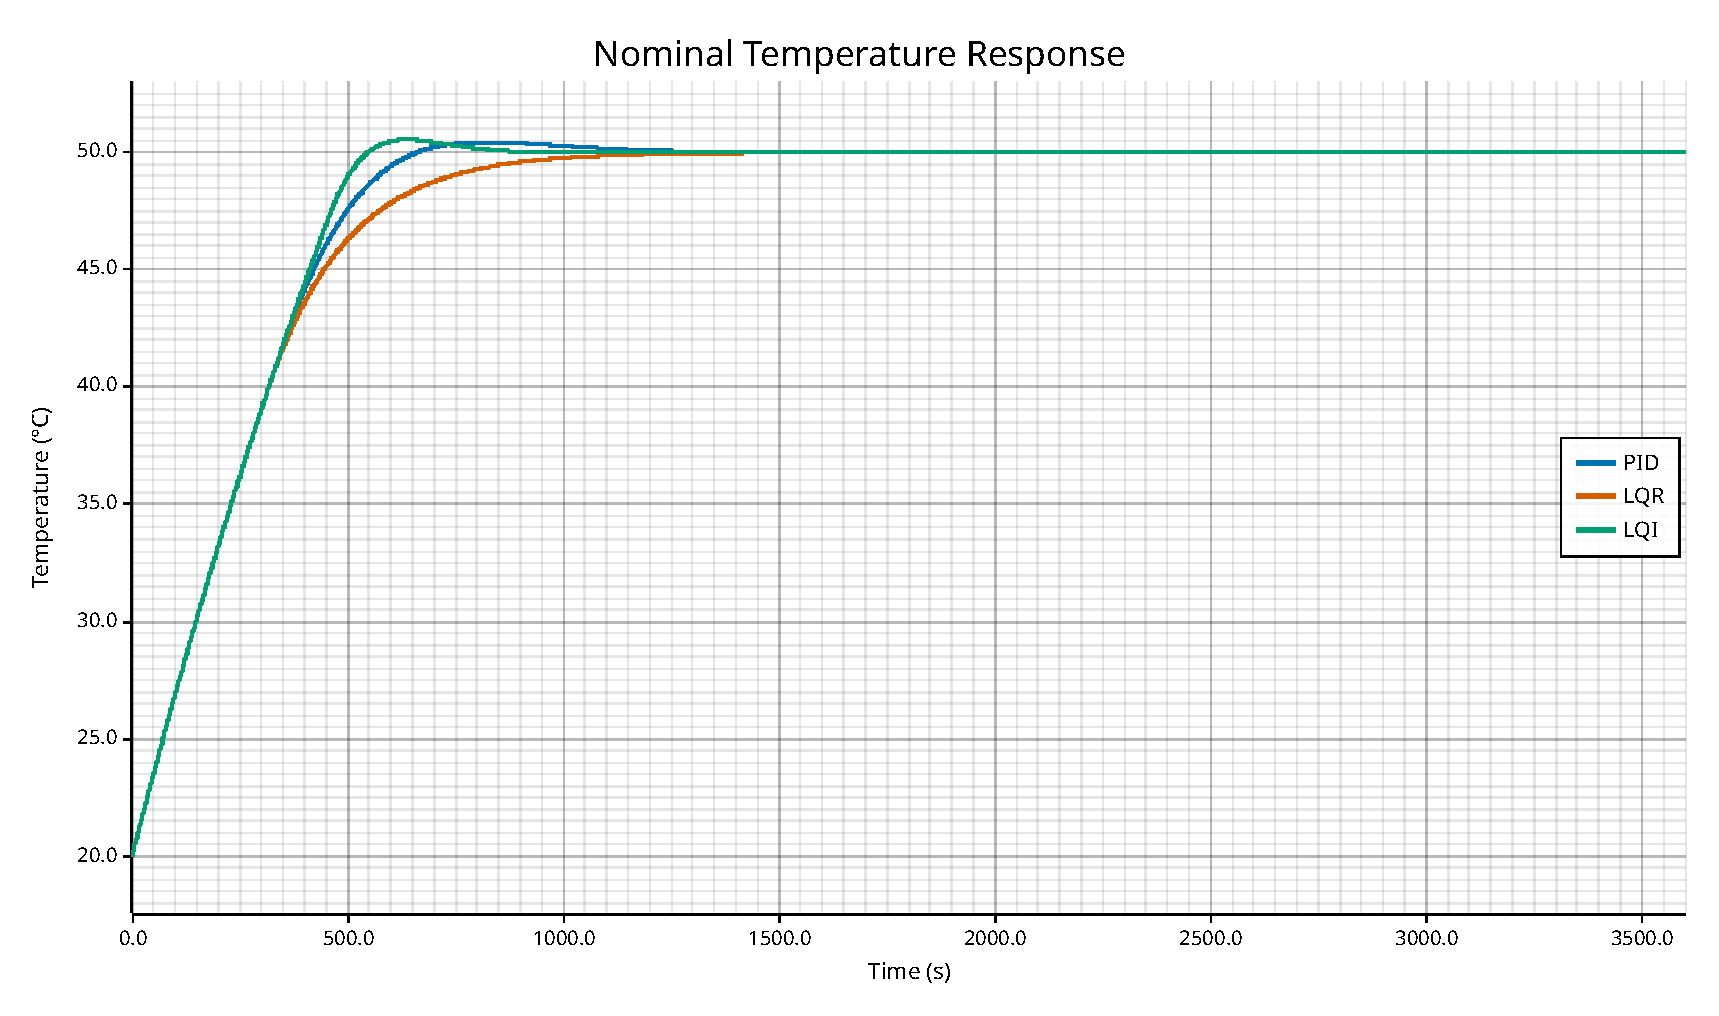
\includegraphics[width=\linewidth]{figures/nominal-temperature.pdf}\caption{Original-controller nominal tracking.}\label{fig:nominal}\end{figure}
\begin{figure}[!htbp]\centering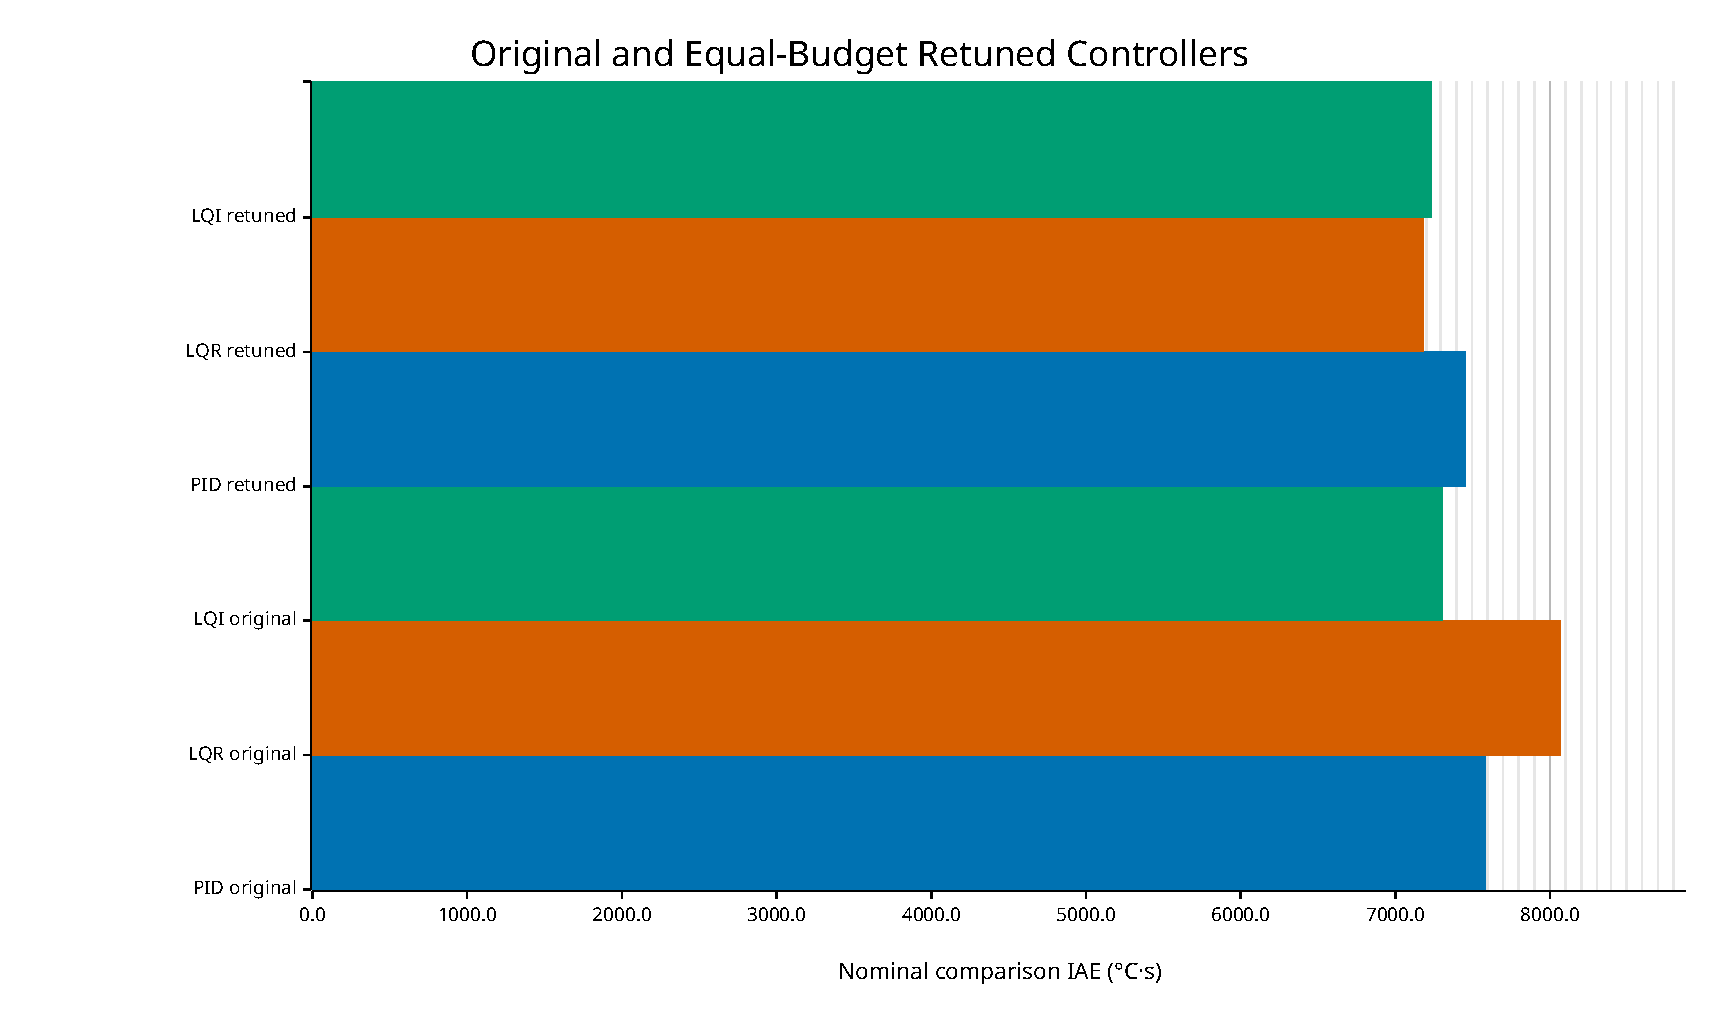
\includegraphics[width=\linewidth]{figures/original-vs-retuned.pdf}\caption{Original versus equal-budget retuned nominal IAE.}\label{fig:tuning}\end{figure}

\subsection{Uncertainty and constant-load rejection}
Capacity uncertainty changes original-controller RMSE ranges by 1.824, 1.898, and \SI{1.878}{\celsius} for PID, LQR, and LQI; equal-percentage $UA$ variation changes them by only 0.196, 0.276, and \SI{0.203}{\celsius}. Capacity therefore dominates this fixed-horizon metric within the tested domain (\cref{fig:uncertainty}).
\begin{figure*}[!t]\centering
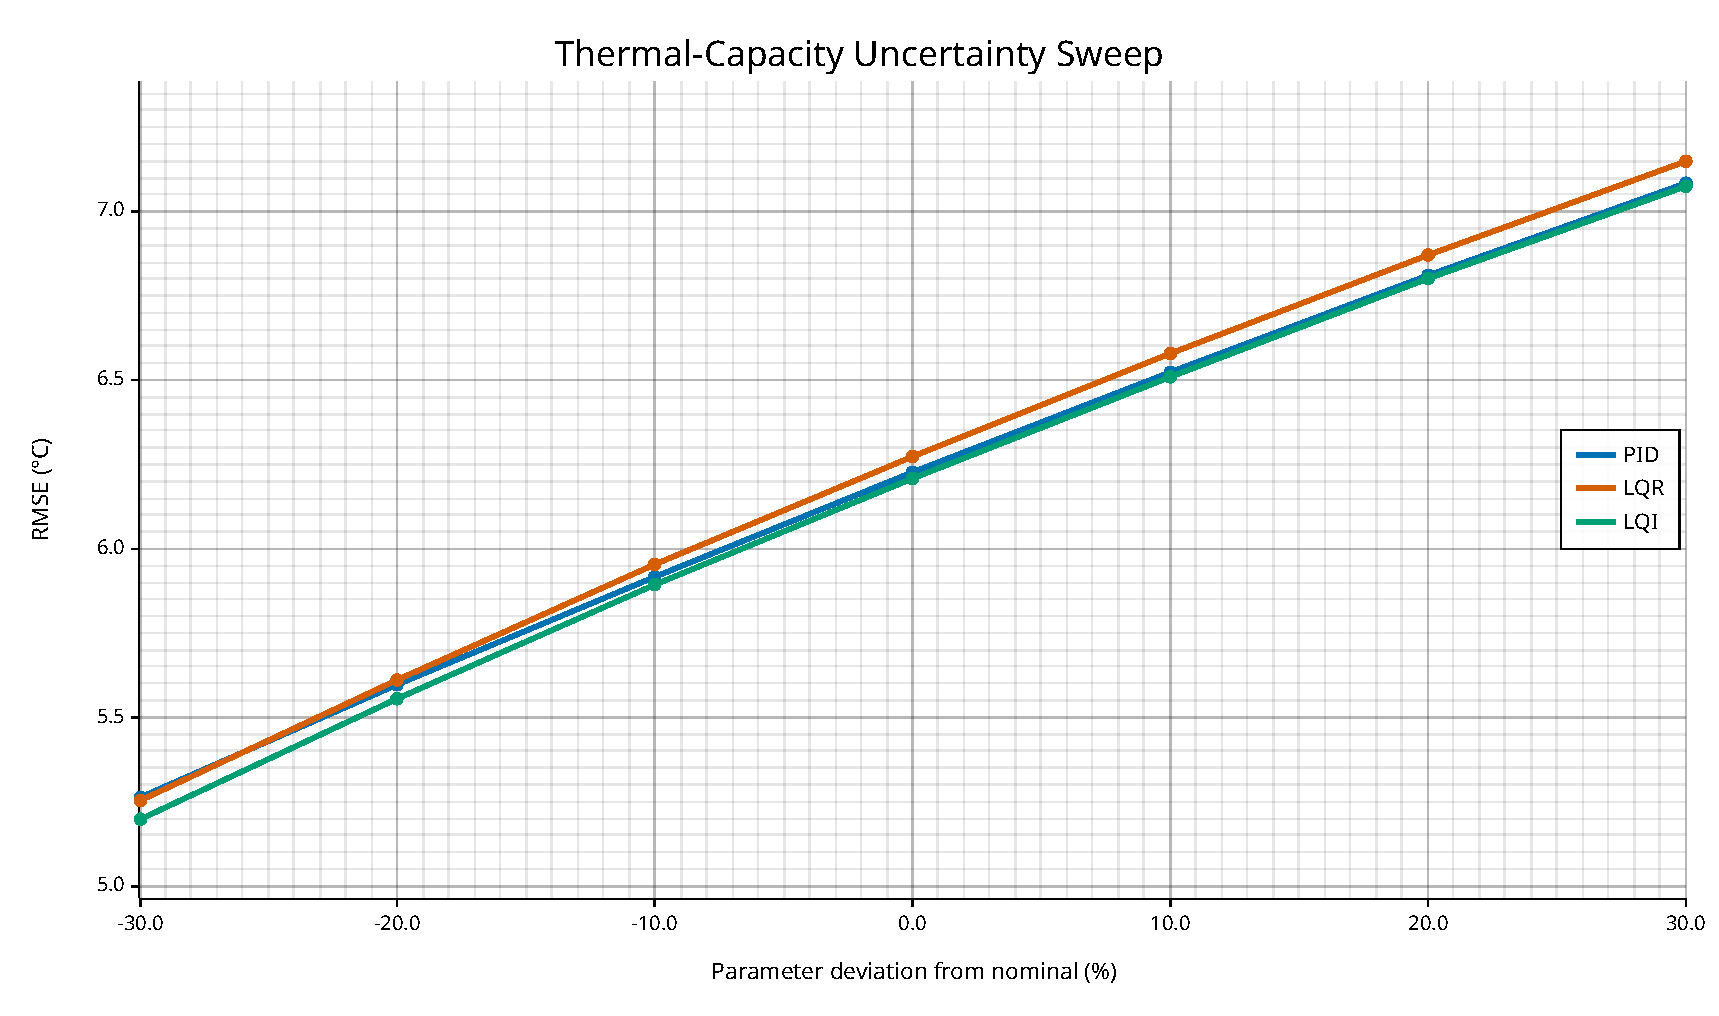
\includegraphics[width=.49\textwidth]{figures/capacity-uncertainty.pdf}\hfill
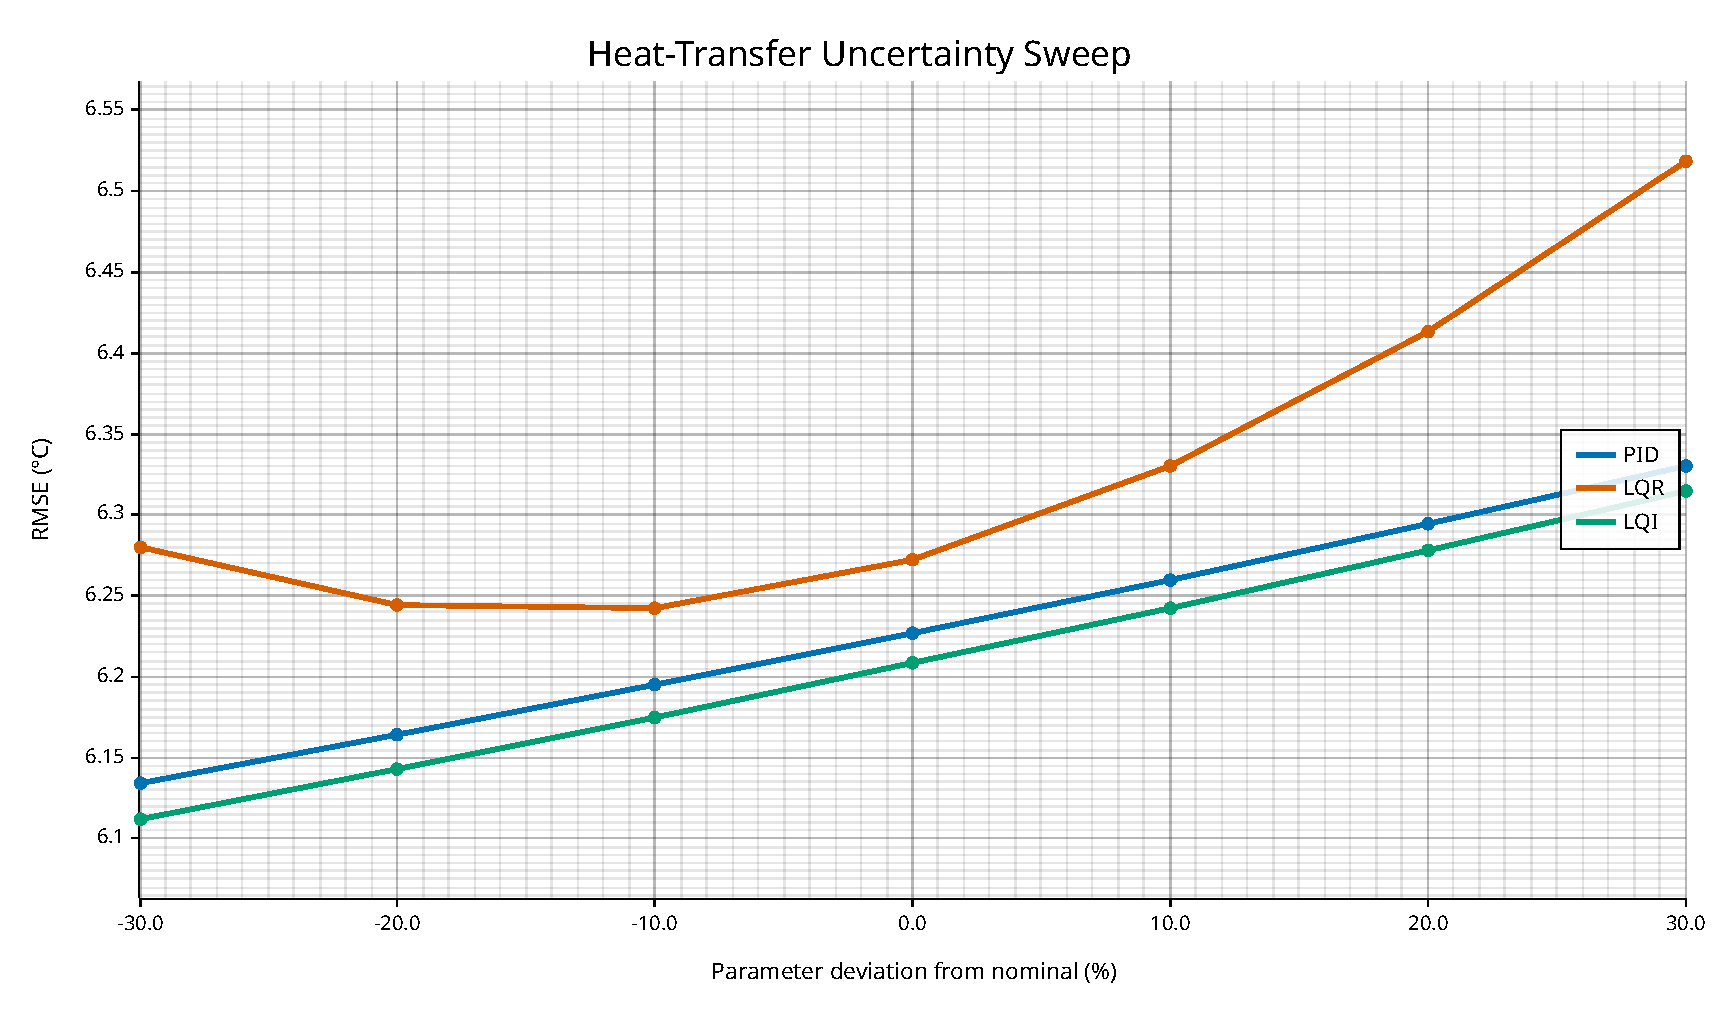
\includegraphics[width=.49\textwidth]{figures/heat-transfer-uncertainty.pdf}
\caption{RMSE sensitivity to isolated thermal-capacity (left) and heat-transfer (right) uncertainty.}\label{fig:uncertainty}\end{figure*}

After the $-\SI{700}{W}$ test load, original-controller post-step IAE is 365.1 (PID), 5006.4 (LQR), and 118.9~$^\circ$C s (LQI). Tail errors are approximately 0, 3.099, and \SI{0}{\celsius}, respectively. Retuned LQR reduces its tail error to \SI{0.079}{\celsius} through much stronger proportional feedback but still lacks structural integral rejection.
\begin{figure}[!htbp]\centering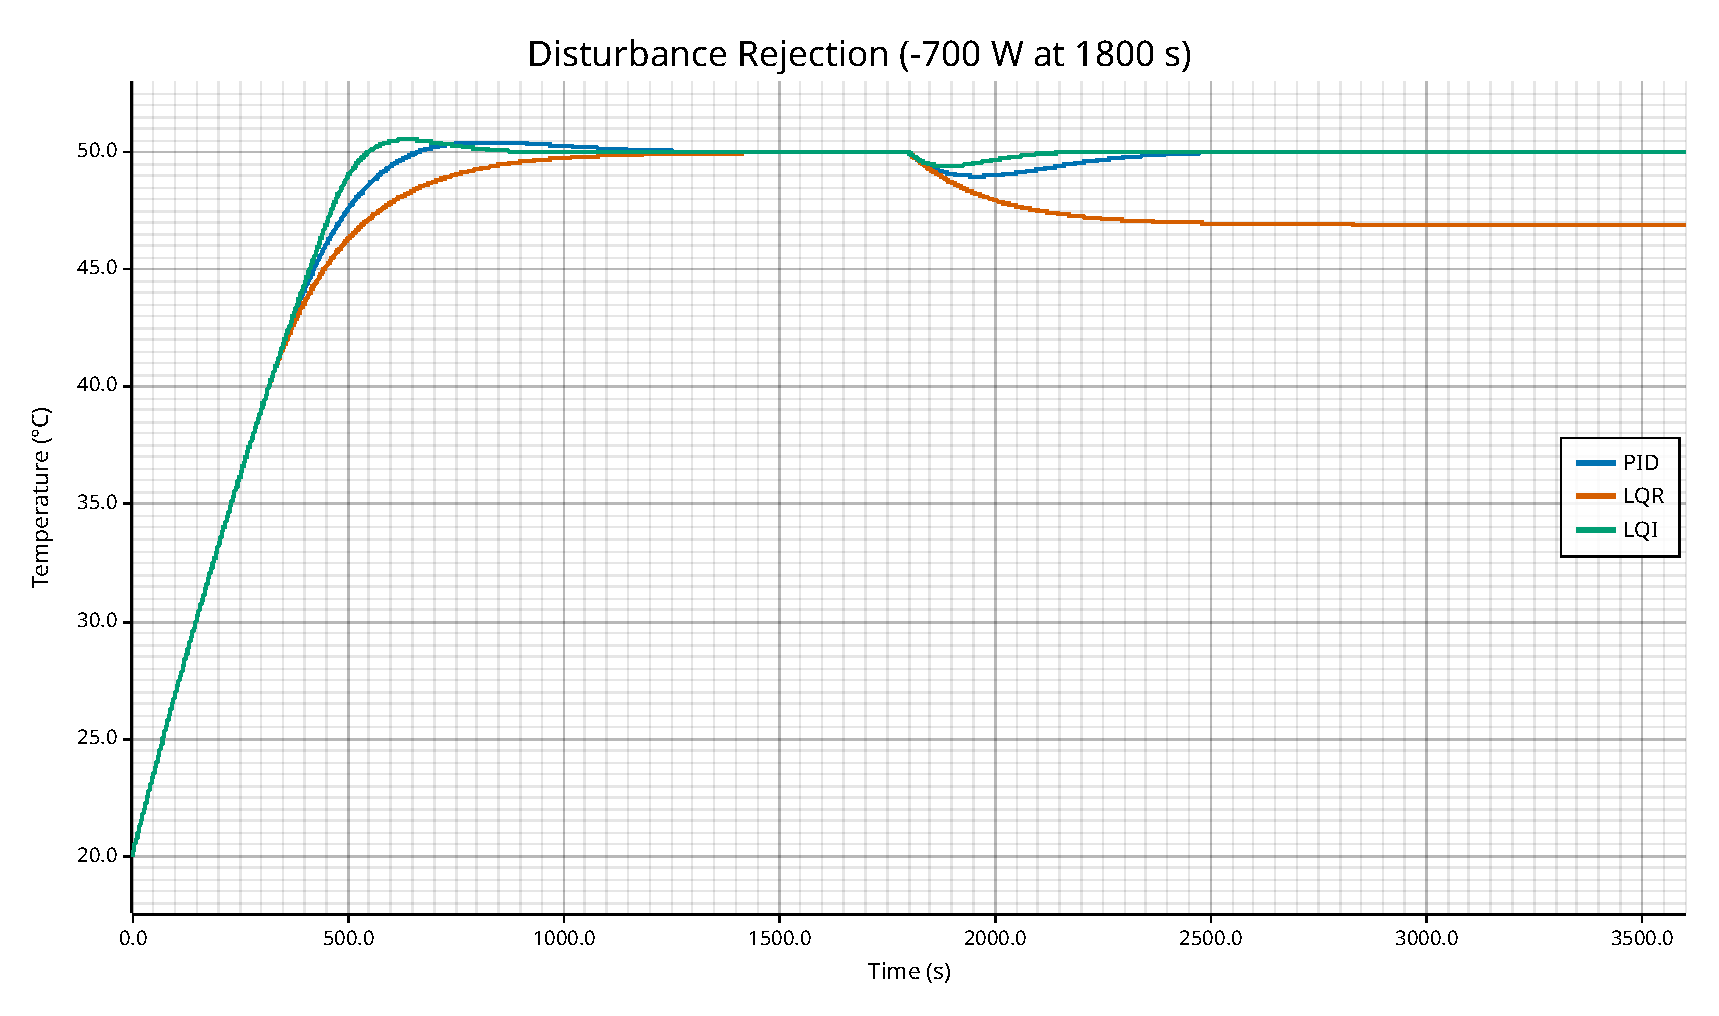
\includegraphics[width=\linewidth]{figures/disturbance-rejection.pdf}\caption{Original-controller response to a $-\SI{700}{W}$ load at \SI{1800}{s}.}\label{fig:disturbance}\end{figure}

\subsection{Saturation and noise}
Corrected original restricted-actuator IAE is 25231.4 (PID), 25268.5 (LQR), and 25209.8~$^\circ$C s (LQI); the original pre-audit claim that LQR won was caused by incorrect anti-windup limits. Retuned restricted-actuator ranking is LQR (25200.3), LQI (25204.6), PID (25221.5), a small ranking change relative to retuned nominal results. Differences are tiny relative to the common saturation-dominated transient.
\begin{figure}[t]\centering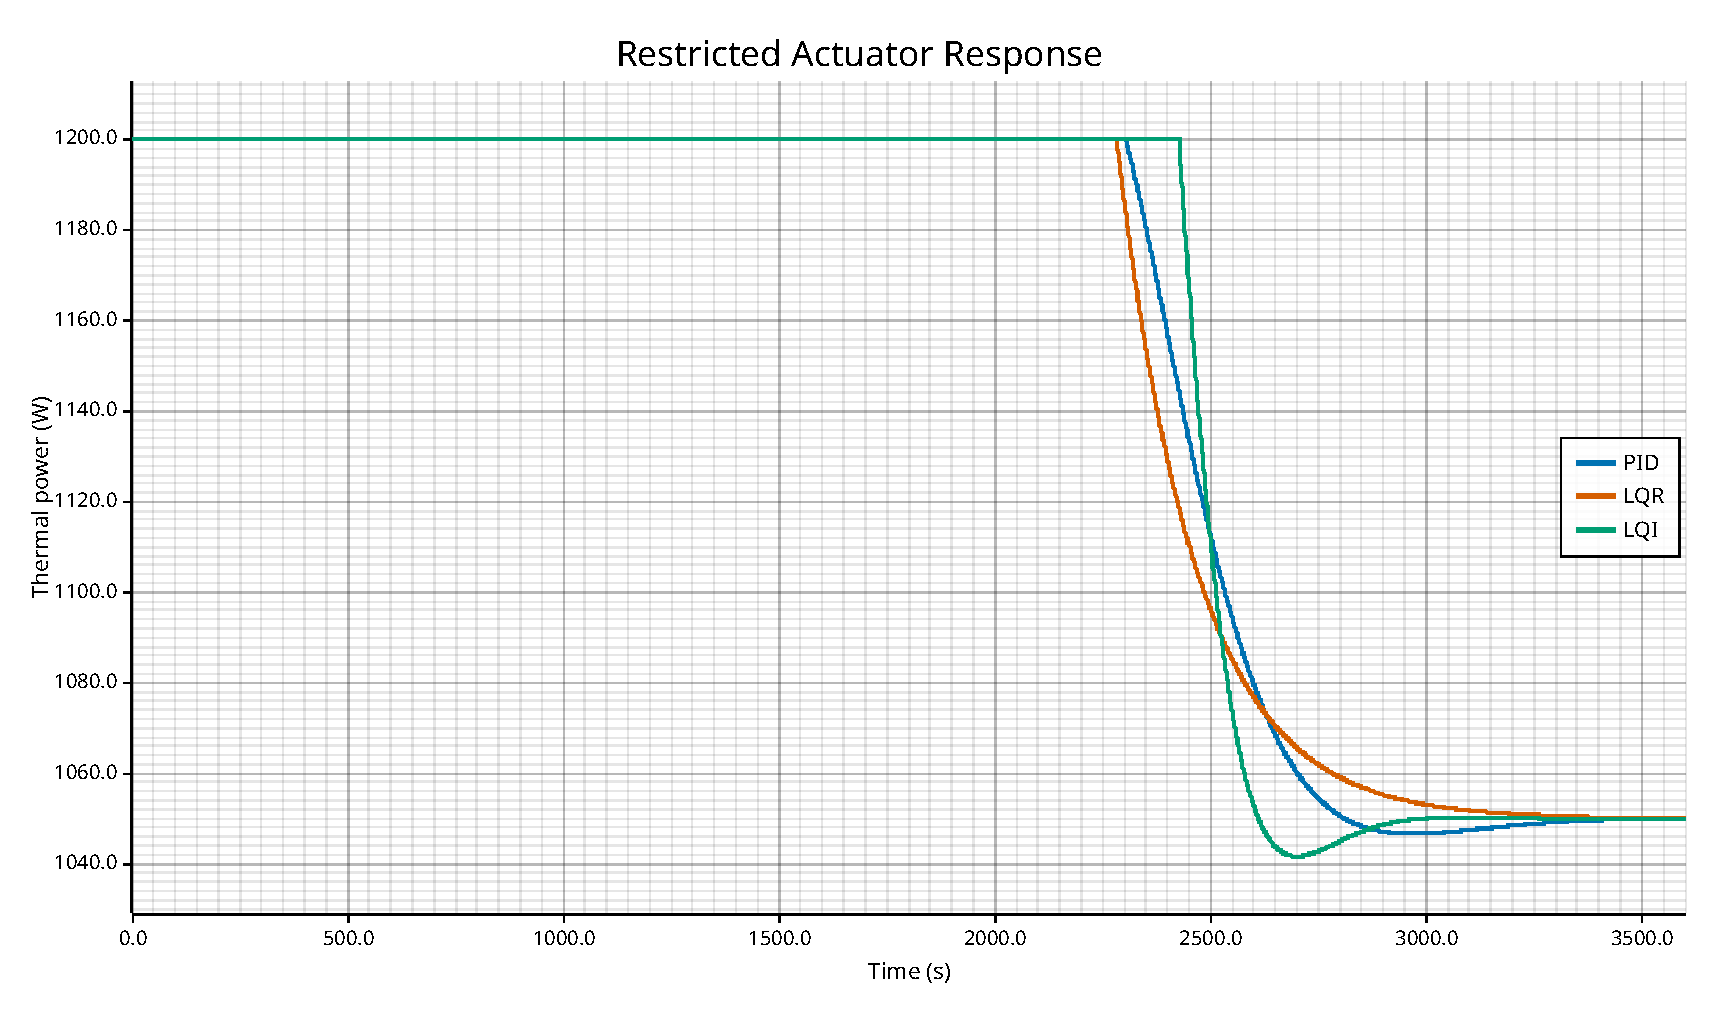
\includegraphics[width=\linewidth]{figures/actuator-saturation.pdf}\caption{Applied power under restricted limits for original controllers.}\label{fig:saturation}\end{figure}

Steady-regime paired LQI-minus-PID noise RMSE is \SI{0.004216}{\celsius} (95\% CI 0.003978--0.004453, $d_z=3.52$). Although standardized against very small replicate variability, four thousandths of a degree is practically negligible for the idealized process. Changing noise magnitude or spectrum may change this conclusion; no broad sensor claim is made.
\begin{figure}[t]\centering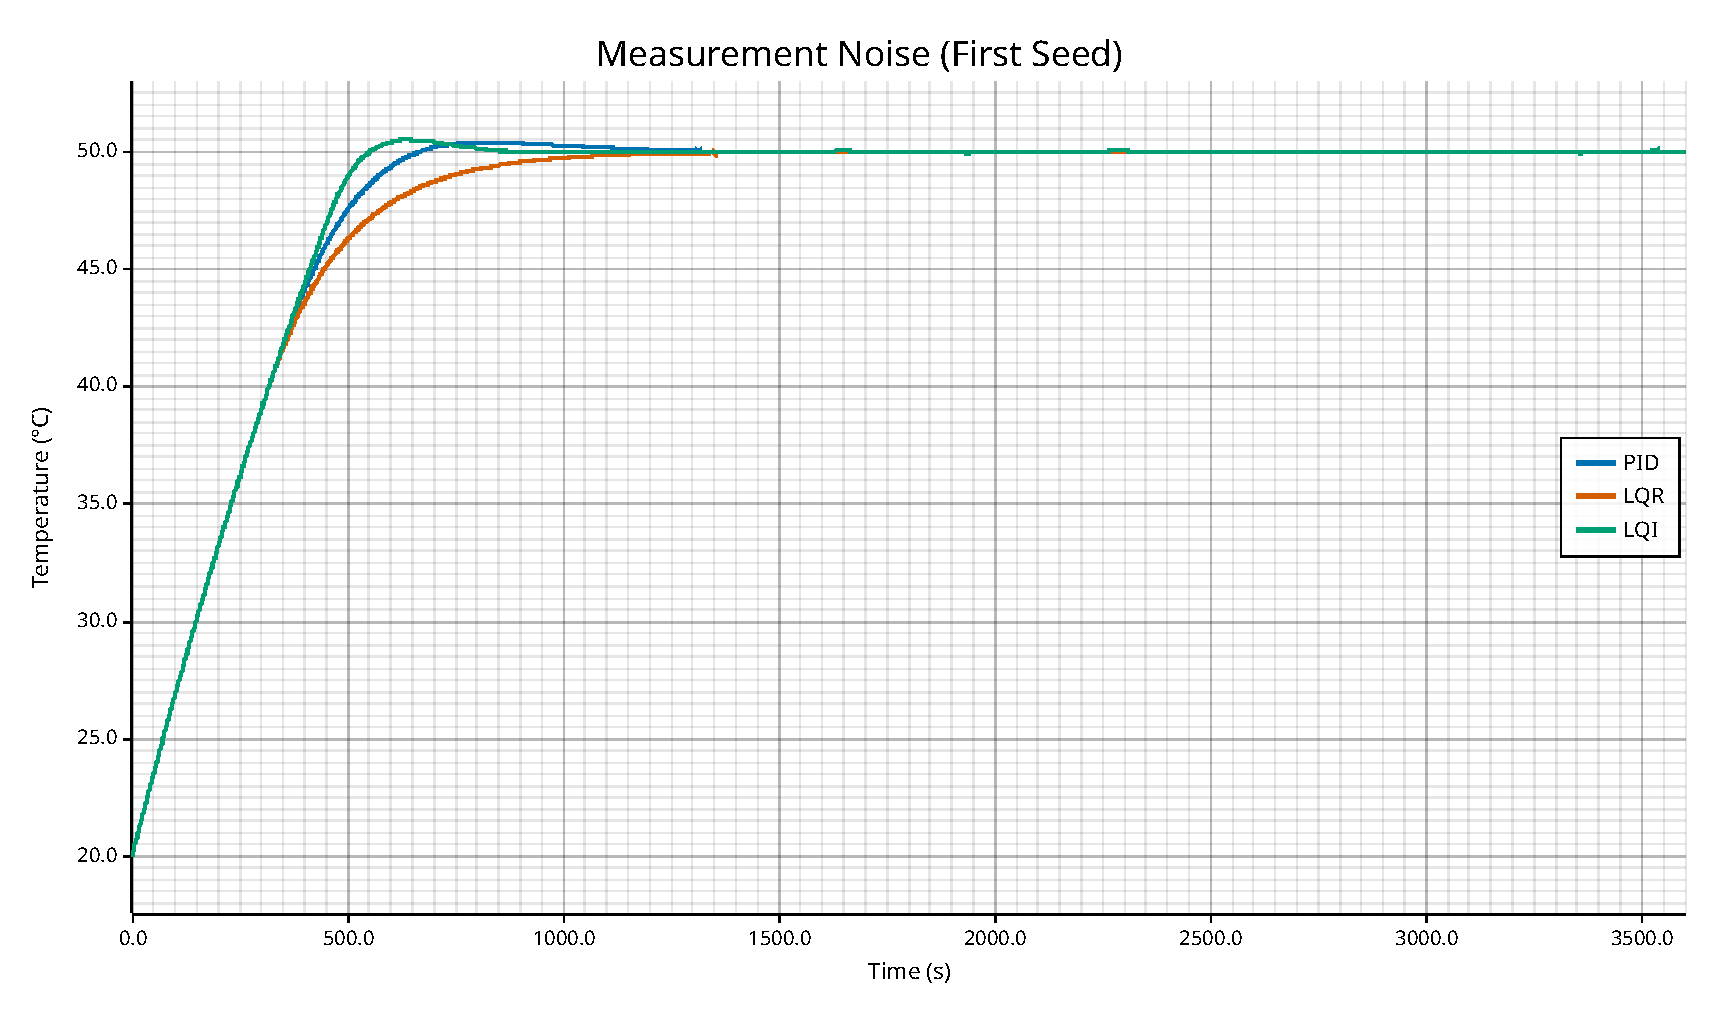
\includegraphics[width=\linewidth]{figures/measurement-noise.pdf}\caption{One paired realization with \SI{0.15}{\celsius} measurement noise.}\label{fig:noise}\end{figure}

\subsection{Unmodeled sensor dynamics}
The lag-and-delay plant exposes a retuning trade-off (\cref{tab:fidelity,fig:fidelity}). Retuned LQR IAE rises to 9345.2~$^\circ$C s, does not settle, and saturates for 2739~s, whereas original LQR IAE is 7804.1. PID and LQI change much less. Aggressive nominal tuning therefore improves the simple plant while reducing tolerance to omitted sensing dynamics.
\begin{table}[!htbp]\centering\caption{Sensor-lag and delay results generated by Rust.}\label{tab:fidelity}\resizebox{\linewidth}{!}{\begin{tabular}{llrrr}\toprule
Design & Controller & IAE ($^\circ$C s) & RMSE ($^\circ$C) & Saturation (s) \\
\midrule
Original & PID & 7447.1 & 6.218 & 365 \\
Original & LQR & 7804.1 & 6.245 & 344 \\
Original & LQI & 7289.2 & 6.208 & 488 \\
Retuned & PID & 7364.1 & 6.215 & 395 \\
Retuned & LQR & 9345.2 & 6.252 & 2739 \\
Retuned & LQI & 7295.1 & 6.208 & 507 \\
\bottomrule\end{tabular}
}\end{table}
\begin{figure}[t]\centering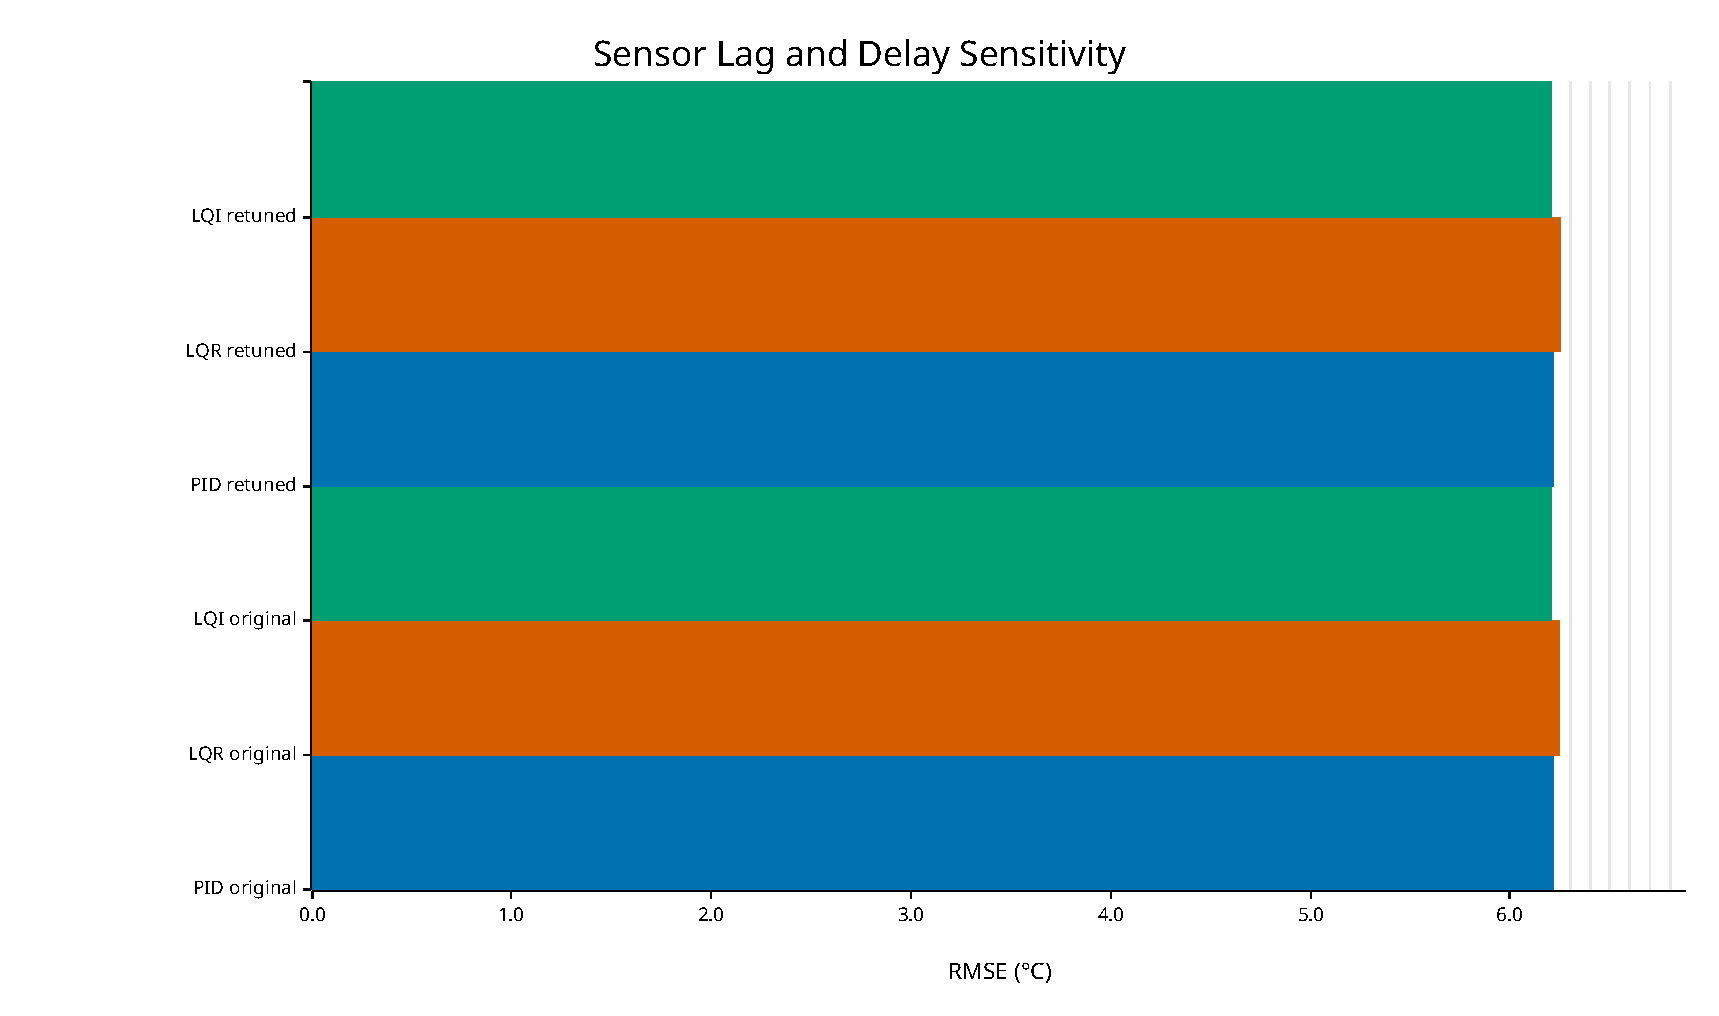
\includegraphics[width=\linewidth]{figures/higher-fidelity-summary.pdf}\caption{RMSE with a \SI{20}{s} sensor lag and \SI{10}{s} delay.}\label{fig:fidelity}\end{figure}
\FloatBarrier


\section{Stability Analysis}\label{sec:stability}
The statements below concern unsaturated, noise-free linear loops. They do not transfer automatically to the saturated nonlinear simulation.

For LQR the uncertain scalar characteristic equation is
\begin{equation}
z-[A_d(C_{\rm th},UA)-B_d(C_{\rm th},UA)K]=0. \label{eq:lqrchar}
\end{equation}
On the continuous box $C_{\rm th}\in[0.7,1.3]C_0$, $UA\in[0.7,1.3]UA_0$, monotonic exponential bounds give intervals for $A_d$ and $B_d$. Natural interval evaluation of \cref{eq:lqrchar} leaves a positive unit-circle margin 0.003961, formally certifying the original LQR for this box.

The LQI closed-loop matrix is
\begin{equation}
F_{\rm LQI}=\begin{bmatrix}A_d-B_dK_x&-B_dK_z\\-h&1\end{bmatrix}. \label{eq:lqimatrix}
\end{equation}
For characteristic polynomial $z^2-tz+\delta$, second-order Jury conditions are $1-t+\delta>0$, $1+t+\delta>0$, and $1-\delta>0$. Validated outward-conservative interval evaluation over $128^2$ covering subboxes gives minimum margins $3.19\times10^{-5}$, 3.95, and 0.0137, respectively. Their positivity certifies original LQI stability throughout the continuous box; subdivision only reduces dependency overestimation and does not omit points.

The implemented PID has a fourth-order linear realization because integral, filtered derivative, and previous measurement are states. Its characteristic equation is $\det(zI-F_{\rm PID})=0$, where $F_{\rm PID}$ is generated directly from the discrete update. A 61-by-61 grid gives spectral radius 0.992397--0.995996, but coefficient dependencies prevent the present interval calculation from proving the full box. Formal PID robust stability therefore remains unproven.
\begin{table}[!htbp]\centering\caption{Formal and gridded stability evidence.}\label{tab:stability}\resizebox{\linewidth}{!}{\begin{tabular}{lcc}\toprule
Controller & Formal interval result & Grid radius range \\
\midrule
PID & Unproven & 0.992397--0.995996 \\
LQR & Certified (margin 0.003961) & 0.991930--0.996039 \\
LQI & Certified (min. Jury margin 0.000032) & 0.986843--0.993128 \\
\bottomrule\end{tabular}
}\end{table}
\begin{figure}[t]\centering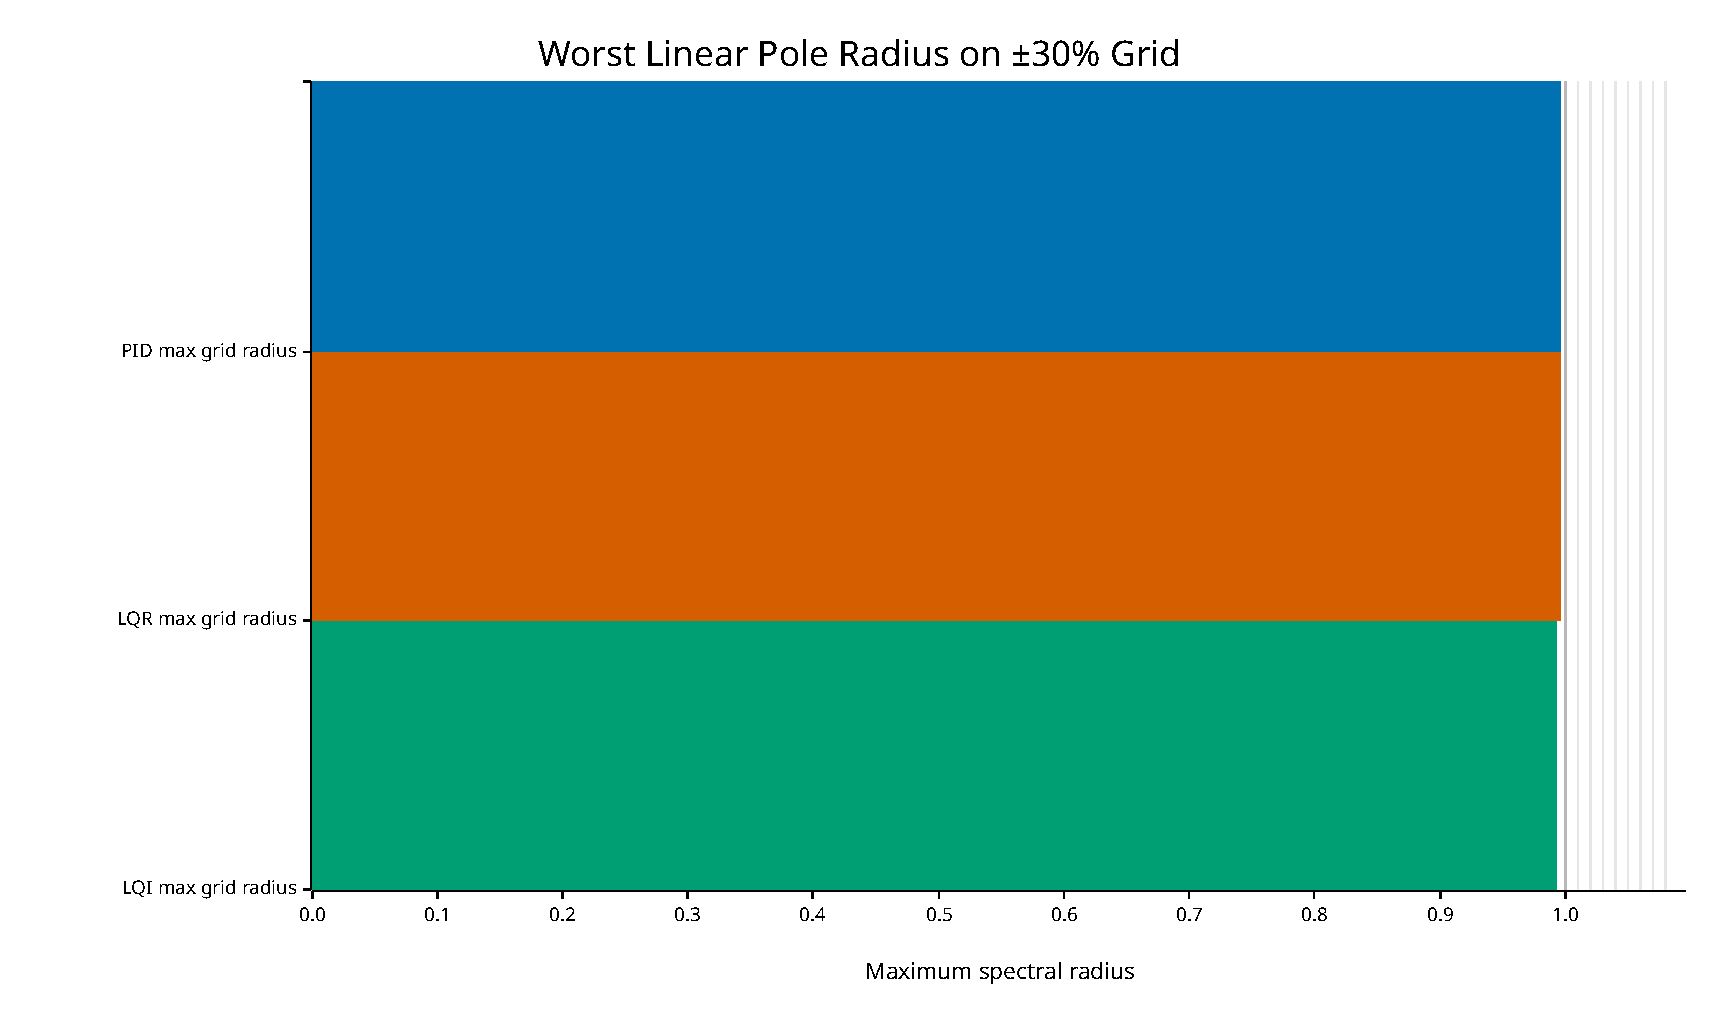
\includegraphics[width=\linewidth]{figures/stability-domain-summary.pdf}\caption{Worst spectral radius on the integer uncertainty grid. This figure is supporting numerical evidence, not the interval proof.}\label{fig:stability}\end{figure}
\FloatBarrier


\section{Discussion}\label{sec:discussion}
The revised evidence separates controller structure from tuning. Original LQI leads nominal tracking and load rejection; equal-budget tuning lets LQR lead the nominal comparison, mainly by selecting very high feedback authority. That advantage is conditional: delayed sensing causes sustained saturation and removes the nominal benefit. Integral action reliably rejects feasible constant thermal loads, but LQI is not uniformly best under noise, saturation, or unmodeled dynamics.

The anti-windup correction is scientifically material. Before correction, PID/LQI integrated against nominal limits while the plant used tighter limits. The corrected result does not support the earlier hypothesis that the restricted actuator makes original LQR best. With retuned gains, LQR narrowly leads the restricted IAE, but differences are practically small and saturation dominates all controllers.

Equal candidate counts and identical scenarios improve fairness but do not equalize optimization difficulty: LQR has two searched weights, PID and LQI have three, and their parameter-to-response maps differ. The result is best viewed as a controlled finite-budget comparison. Likewise, statistical confidence under independent Gaussian realizations quantifies Monte Carlo precision, not uncertainty in real sensor physics or plant parameters.

The chemical role is intentionally limited. The model expresses solution heat capacity, heat transfer, and thermal equilibrium for a non-reactive liquid. No claim is made about reactor kinetics, concentration, industrial equipment, or laboratory validation.


\section{Limitations}
Parameters are illustrative; there are no physical measurements. Perfect mixing, constant properties, linear heat loss, instantaneous actuation, and Gaussian white sensor noise are simplifying assumptions. The secondary model adds sensor lag and delay but is not a validated industrial model. Only LQR and LQI receive formal continuous-box certificates; PID has dense-grid evidence. Saturated stability is not proved. The tuning budget is equal in evaluation count rather than search complexity, and nominal comparison overlaps the training scenario. Confidence intervals assume independent pseudorandom streams under one noise distribution. The study therefore supports conditional computational conclusions only.


\section{Conclusion}
This audited simulation study shows that controller rankings depend on objective, mismatch, and omitted dynamics. Equal-budget tuning changes nominal ranking from LQI--PID--LQR to LQR--LQI--PID, while a modest sensor lag and delay remove the tuned LQR advantage. Integral action provides the clearest constant-load benefit. Capacity uncertainty affects fixed-horizon RMSE more strongly than equal-percentage heat-transfer uncertainty. Correct saturation plumbing invalidates the original negative finding, and noise differences are statistically clear but practically small. Interval analysis proves unsaturated robust stability over the declared continuous parameter box for original LQR and LQI, while PID and all saturated loops retain explicitly limited evidence. The repository provides a reproducible computational manuscript, not a novel control algorithm or physical-process validation. Future work can remain simulation-only by extending interval analysis, delay-robust tuning, colored-noise models, and higher-order thermal networks.

\section*{Reproducibility Statement}
All executable research code is Rust. The repository pins Rust 1.100.0 and dependency versions, records configurations and seeds, generates tables and vector figures from computed results, and rebuilds this paper with the supplied template workflow. The complete study is reproduced with \texttt{cargo run --release -- run-all} followed by \texttt{make} in \texttt{paper/}.

\printbibliography
\end{document}
